\documentclass[12pt]{exam}
\usepackage{booktabs}
\usepackage[hmargin=1.5cm, top=1.5cm, bottom=2cm]{geometry}
\usepackage[T1]{fontenc}
\usepackage[utf8]{inputenc}
\usepackage[portuguese]{babel}
\usepackage{graphicx}
\usepackage{tikz}
\usepackage{titling}
\usepackage{indentfirst}
\usepackage{subcaption}
\usepackage{enumitem}
\usepackage{pifont}
\usepackage{siunitx}
\usepackage{adjustbox}
\usepackage{hyperref}
\usepackage{interval}
\usepackage{microtype}
\usepackage{amsmath}

\graphicspath{ {./output} }
\setlength{\droptitle}{-5em}
\renewcommand\_{\textunderscore\linebreak[1]}
\cfoot{\normalsize\thepage}

\author{Grupo: al020\\Alunos: Duarte Almeida (ist195565) e Gustavo Aguiar (ist195587)}
\title{Numbrix IA P3 2021/2022}
\date{}\date{}

\begin{document}
    \maketitle
    \begin{tikzpicture}[overlay, remember picture]
        \node[xshift=3.5cm,yshift=-2cm] at (current page.north west) {
\includegraphics[scale = 0.35]{logo_ist.jpeg}};
    \end{tikzpicture}
    \vspace{-6em}
    \section{Descrição do Problema e da Solução}
    \indent O presente relatório apresenta uma solução para o problema \textit{Numbrix}.
    Neste existe uma grelha \textbf{$N\times N$}, onde cada célula pode conter um número positivo inteiro entre $1$ e $N^2$.
    O objetivo é preencher a grelha com todos os números de $1$ a $N^2$ por forma a que formem uma sequência de números adjacentes horizontal ou verticalmente. \par

    \indent A solução formaliza o \textit{Numbrix} como um problema de procura. Cada \textbf{estado} \textit{state} é representado por uma matriz $N \times N$, $state.board$, sendo que \textit{estado inicial} é uma representação matricial do tabuleiro dado inicialmente. Dado um estado, as \textbf{ações} aplicáveis correspondem a colocar um número numa posição livre (i.e., nula) adjacente à posição com maior número na sequência de um ou mais números adjacentes com os menores valores das presentes no tabuleiro. Por exemplo, as ações aplicáveis ao tabuleiro (a) abaixo consiste em preencher $state.board[0][1]$ com 3 (considerando-se que os índices das linhas e colunas começam em 0). Se esse número for $N^2$ (caso (b)) as ações aplicáveis consiste em atribuir o antecessor à posição com o menor número na (única) sequência de números adjacentes (i.e., preencher $state.board[1][2]$ ou $state.board[0][1]$ com 4).
        \begin{table}[ht!]\centering\footnotesize
            \begin{subtable}{0.2\textwidth}
                \centering
                \begin{tabular}{ccc}
                    2 & 0 & 4 \\
                    1 & 0 & 5 \\
                    0 & 0 & 0
                \end{tabular}
                \caption{}
            \end{subtable}
            \begin{subtable}{0.2\textwidth}
                \centering
                \begin{tabular}{ccc}
                    0 & 0 & 0 \\
                    6 & 5 & 0 \\
                    7 & 8 & 9
                \end{tabular}
                \caption{}
            \end{subtable}
        \end{table}

        \indent O \textbf{resultado} de uma \textbf{ação} $(position = (x, y), value)$ consiste em criar um novo estado $state'$ copiando o estado do nó pai, procedendo-se em seguida à atribuição $state'.board[x][y] = value$.

        \indent Por forma a guiar eficientemente a procura, formulou-se a seguinte \textbf{heurística} parametrizada $h_\alpha$, que vale $\infty$ se (1) não existe uma sequência de posições livres entre a posição com maior número na sequência de um ou mais números contíguos com os menores valores das presentes no tabuleiro e a posição com o menor valor da sequência com menores números entre as restantes; (2) se a distância de \textit{Manhattan} entre estas duas posições é superior ao valor absoluto da diferença entre os seus valores; (3) se há pelos menos $min - 1$ e $N^2 - max$ posições livres atingíveis da posição com menor $min$ e maior valor $max$ presentes no tabuleiro, resp; ou (4) se qualquer conjunto de posições livres adjacentes possui pelo menos duas posições com \textbf{valores maiores} que o maior valor já atribuído mas que \textbf{não são sucessores} (tal é uma condição necessária para que esses espaços sejam posteriormente utilizados no futuro). Caso contrário, sendo $F$ o conjunto de posições vagas no tabuleiro, e $adj(pos)$ o conjunto de posições livres adjacentes à posição $pos$, tem-se:
        \vspace*{5mm}
        \[
            h_\alpha = \sum_{pos \in F} (4 - |adj(pos)|)^\alpha
            \]
        \indent O \textbf{teste objetivo} consiste em determinar se só existe uma sequência de números contíguos no tabuleiro, cujo o máximo é $N^2$ e o mínimo é 1 (variáveis que se podem manter em memória). O \textbf{custo de cada ação} é 1.
    
    \pagebreak

    \section{Implementação e Análise dos Resultados}~
        \indent Dados os testes de \textit{input/output} fornecidos pelo corpo docente, obtiveram-se os seguintes resultados aplicando o algoritmo implementado:\\

        \begin{adjustbox}{width={\textwidth}, totalheight={\textheight}, keepaspectratio}
        \begin{tabular}{l cccc cccc cccc}
        \toprule
         & \multicolumn{4}{c}{Tempo de Execução (s)} & \multicolumn{4}{c}{Nós Gerados} & \multicolumn{4}{c}{Nós Expandidos}\\
        \cmidrule(lr){2-5} \cmidrule(lr){6-9} \cmidrule(lr){10-13}
        Input           & BFS  & DFS  & A* & GS       & BFS  & DFS  & A* & GS        & BFS  & DFS  & A* & GS \\
        \midrule
        1               & 0.0004 & 0.0003  & 0.0008    & 0.0008            & 10    & 7 & 7    & 7       & 10   & 5   & 5      &5  \\
        2               & 0.4837 & 0.1165  & 0.3179    & 0.3314            & 7280  & 1218 & 779  & 834       & 7270   & 1199   & 493    &516  \\
        3               & 0.0852 & 0.0360  & 0.0158    & 0.0147            & 2186  & 991 & 59   & 54       & 2184   & 980   & 34     &32  \\
        4               & 0.3192 & 0.1758  & 0.0630    & 0.0611            & 4473  & 2898 & 230  & 230       & 4473   & 2887   & 118    &118  \\
        5               & 0.2385 & 0.0176  & 0.1479    & 0.0454            & 5760  & 430 & 516  & 188       & 5760   & 420   & 302    &107  \\
        6               & 0.1693 & 0.0633  & 0.1000    & 0.0998            & 2857  & 1092 & 199  & 199       & 2857   & 1076   & 111    &112  \\
        7             & 106.1534 & 39.4617  & 0.4971    & 0.3778         & 1343928  & 714831 & 928  & 744       & 1343928   & 714802   & 437    &365  \\
        8               & 0.5891 & 0.2635  & 0.4280    & 0.4117            & 4611  & 2653 & 599  & 588       & 4584   & 2634   & 386    &380  \\
        9               & 0.6193 & 0.2668  & 0.4232    & 0.4134            & 4611  & 2653 & 599  & 588       & 4584   & 2634   & 386    &380  \\
        10              & 0.1804 & 0.0536  & 0.2072    & 0.1835            & 2303  & 957 & 338  & 312       & 2303   & 943   & 232    &215  \\
        \bottomrule
        \end{tabular}
        \end{adjustbox} \\
        
        \indent Todos os métodos de procura são \textbf{completos}, dado que, por construção, a solução do problema fica a uma profundidade máxima de $N^2$, nunca se gerando estados repetidos dado que se vão atribuindo números por ordem crescente. Em particular, obtém-se uma complexidade temporal e espacial de $O(4^{N^2})$. A performance superior da DFS deve-se ao facto de todos os nós expandidos por DFS em relação à BFS também serem expandidos por BFS. A utilização de um heurística melhora substancialmente os tempos em relação aos dois algoritmos anteriores (confere caso com $n$ = 7), dado que o seu valor está correlacionado com a usabilidade dos espaços livres restantes (reforçando a condição (4) exposta na heurística). Para determinar o seu valor ótimo de $\alpha$, geraram-se 6 instâncias de tabuleiros $10 \times 10$ e utilizaram-se ambos os algoritmos com a mesma heurística, com incrementos de $0.2$ no expoente da heurística, $\alpha$, tal que $\alpha \in \interval{1}{2}.$
        \vspace{-4.5mm}
        \begin{figure}[ht!]
        \centering
        \subfloat[\centering \textit{A-Star Search}]{{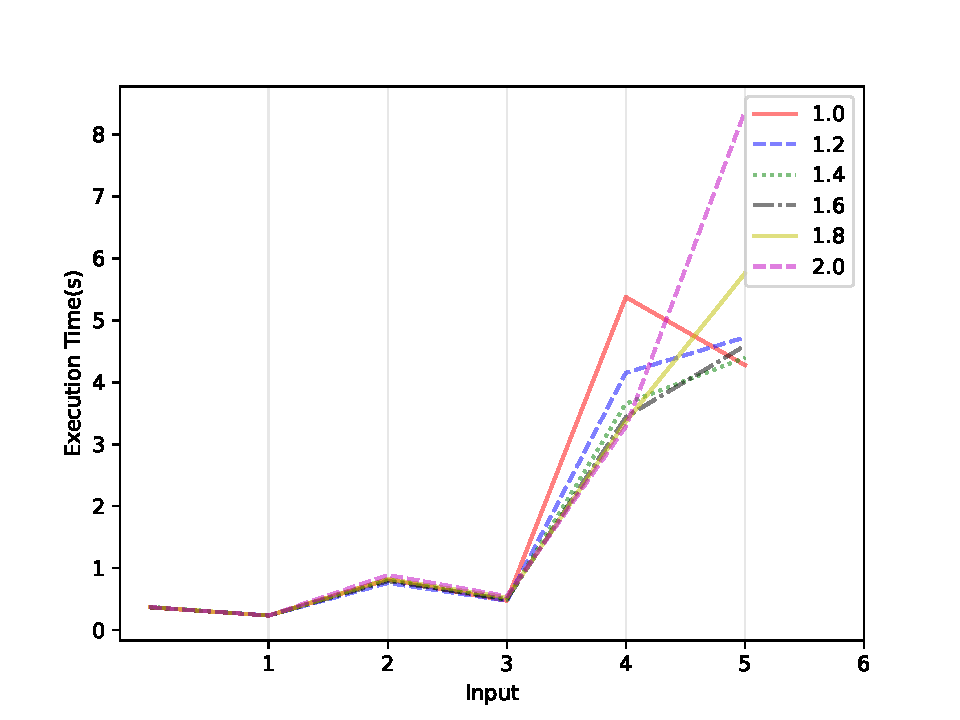
\includegraphics[width=8.5cm]{a-star_h_plot.pdf} }}%
        \qquad
        \subfloat[\centering \textit{Greedy Search}]{{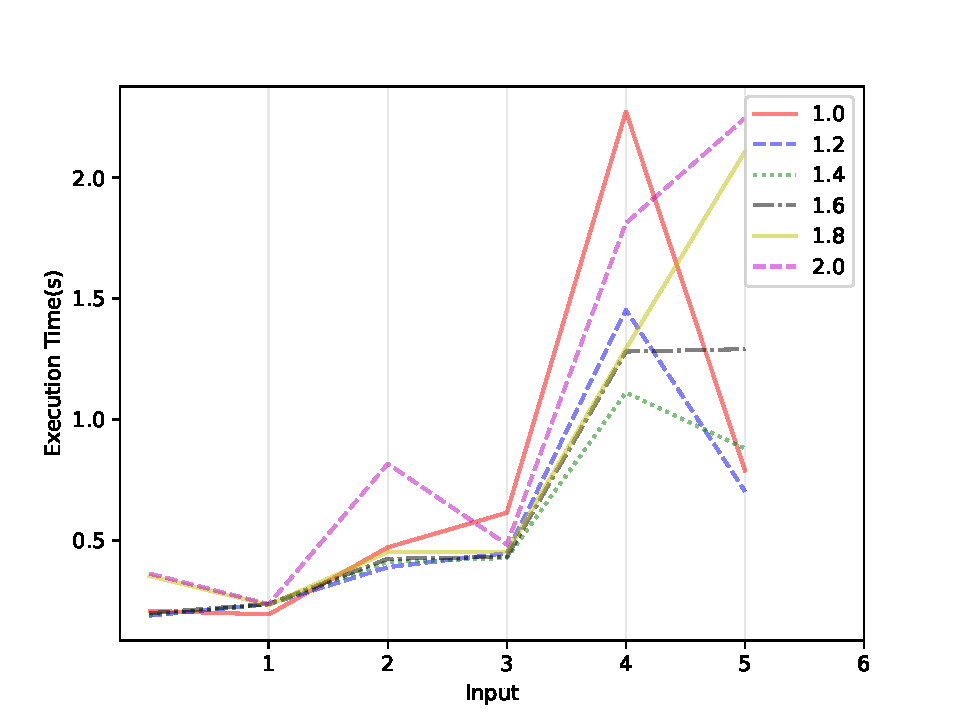
\includegraphics[width=8.5cm]{greedy_h_plot.pdf} }}%
        \label{fig:example}%
        \end{figure}

        \indent Atendendo aos dados obtidos, decidiu-se optar pela implementação com \textbf{procura informada que usa \textit{Greedy Search} e $\alpha$ = 1.4 }. Dado que $\alpha$ controla o decaimento da função heurística para o nó sucessor (que é maior quanto maior for $\alpha$), e que a introdução de uma parcela linear com a profundidade do nó no algoritmo $A^*$ reduz esse decaimento, postula-se que a escolha obtida proporciona um valor optimal da profundidade de cada backtrack realizado.

\end{document}
